\chapter{Fit Probability}
\label{chap:apdx_fitprob}
In Sec.~\ref{sec:weights_tightsel} we use the distribution of $\chi^2_\text{DTF}$ of a \gls{dtf} to suppress combinatorial background.
An interesting transformation of the $\chi^2_\text{DTF}$ distribution is achieved via the regularized upper incomplete gamma function
\begin{equation}
    \label{eq:fitprob}
    \chi^2 \mapsto \frac{1}{\Gamma \left(\text{DoF}/2 \right)} \; \int\limits_{\chi^2/2}^{\infty} \! \mathrm{d}t \, t^{\text{DoF}/2 - 1} \mathrm{e}^{-t} \,,
\end{equation}
where $\Gamma(s)$ is the complete gamma function.
The result of this transformation, which we refer to as the \textit{fit probability} $\operatorname{Prob}(\chi^2, n)$, is the probability that an observed  $\chi_\text{obs}^2$ exceeds the value $\chi^2$ by chance, even for a correct model.
The fit probability itself is distributed uniformly for $\chi^2$-distributed events with $\text{DoF}$ degrees of freedom.

\begin{figure}[htbp]
    \centering
    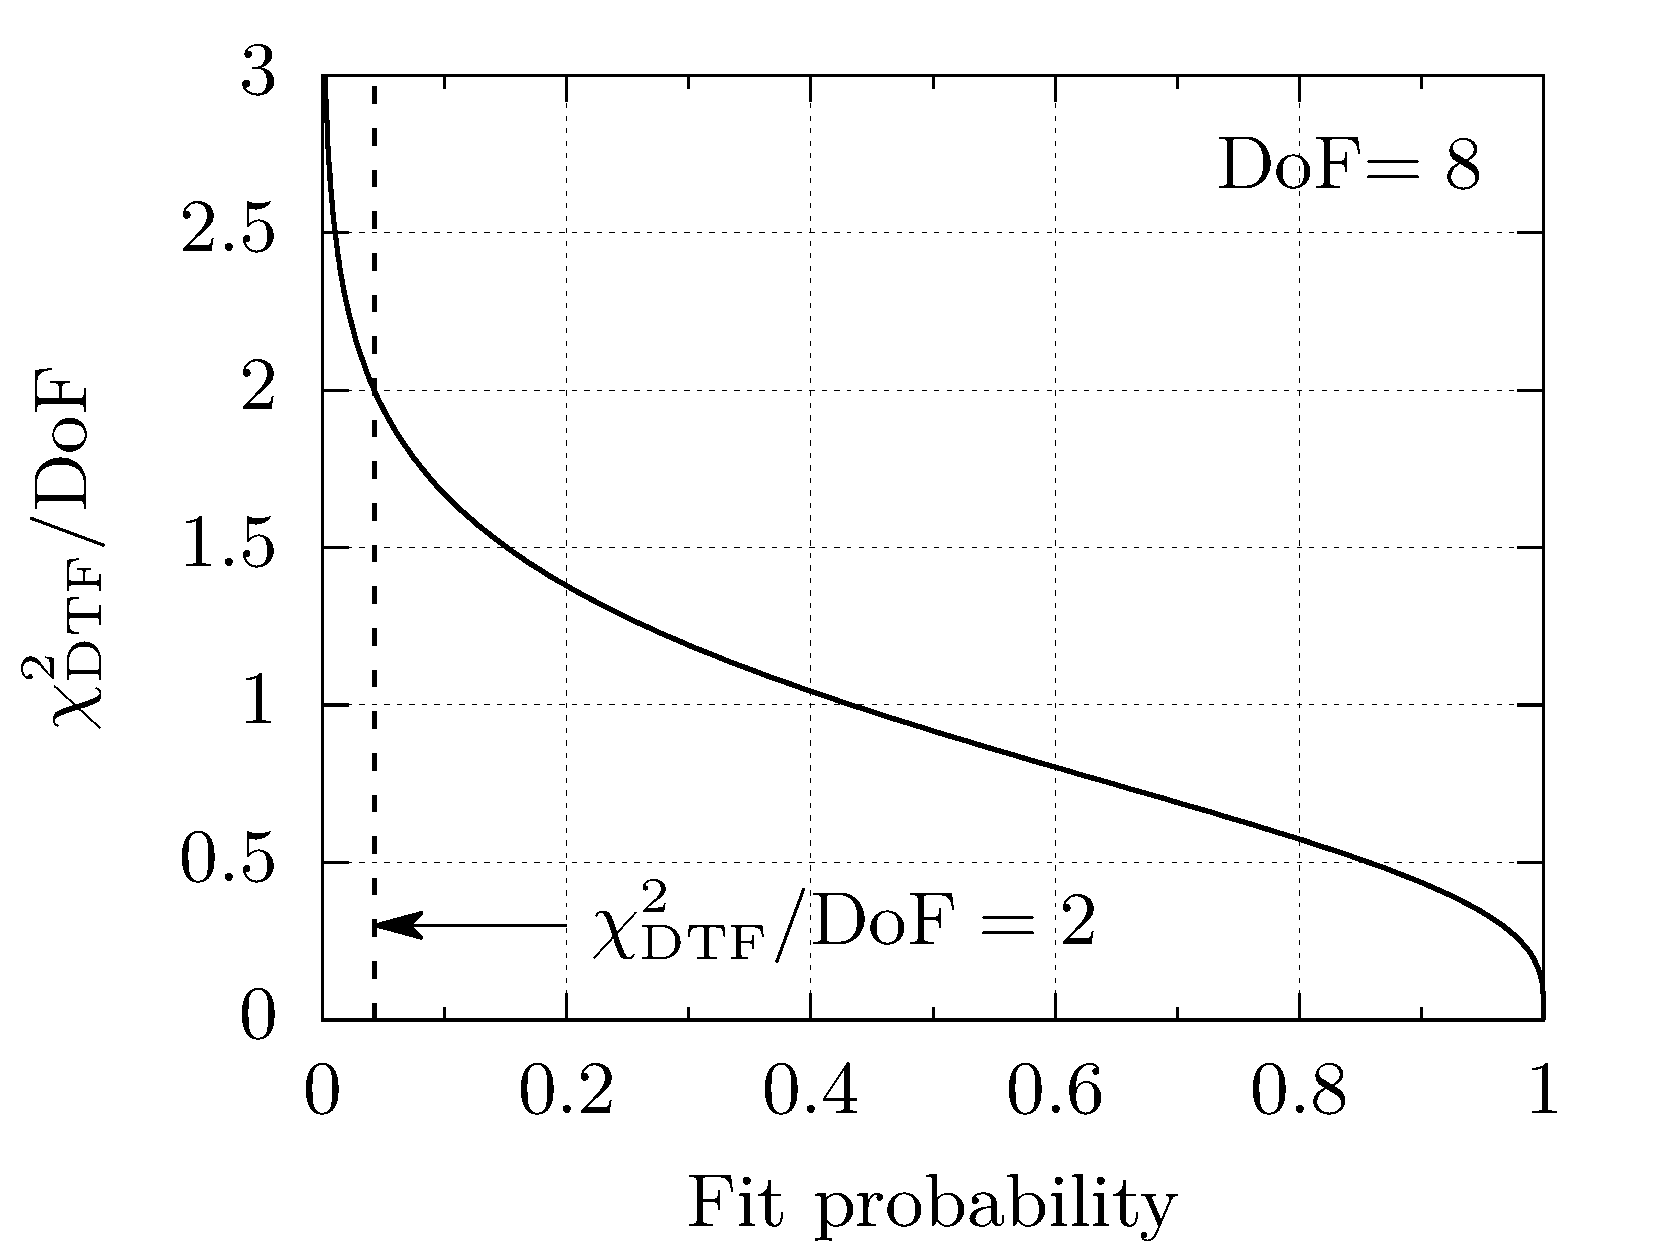
\includegraphics[scale=1.]{Lb2JpsiLz_weighting/fitProb_vs_chi2pndof.png}
    \caption{Fit probability as a function of $\chi^2$ with $8$ \gls{dof} as defined in Eq.~\eqref{eq:fitprob}.}
    \label{fig:fitprob_vs_chi2}
\end{figure}

For the selection requirements of the established tight selection of \decay{\Lb}{\jpsi\Lz} decays, $\chi^2_\text{DTF} / \text{\gls{dof}} = 3$ ($2$) for \gls{LL} (\gls{DD}) tracks with $\text{\gls{dof}} = 8$ (\cf{}~Fig.~\ref{fig:fitprob_vs_chi2}), the inverted fit probability is
\begin{align*}
    1 - \operatorname{Prob}(3 \times 8, 8) &= 99.8\,\% \,, \\
    1 - \operatorname{Prob}(2 \times 8, 8) &= 95.8\,\% \,. \\
\end{align*}
These numbers do not reproduce those found in data (\cf{}~Tab.~\ref{tab:LbToJpsiLz_tighsel_eff}) and thus
$\chi^2_\text{DTF} / \text{\gls{dof}}$ is not exactly $\chi^2$-distributed with $8$ \gls{dof}.
In Fig.~\ref{fig:fitprob_LbToJpsiLz} we show the fit probability distribution of \gls{LL} and \gls{DD} tracks, and for recorded data and (\gls{truthmatched}) simulated events.
Although none of these distributions are flat as expected from a $\chi^2$-distribution, there is no significant discrepancy between recorded data and simulated events visible.\footnote{In Appx.~\ref{chap:apdx_mva_xcheck} we discuss the effect of deviations for large $\chi^2$ values. These deviations are a nuisance for efficiency estimations, but not for the estimation of the calibration factors.}
The reason for the deviation from the expected uniform distribution at small fit probability values is unclear.
Small fit probability values mean large $\chi^2$ values such that the accumulation at small fit probability values translates into too many \glspl{dtf} with large $\chi^2$ values, \ie{}, deviations of a Gaussian shape that raises $\chi^2$-tail contributions.

There are two main reasons which could potentially cause accumulations at small fit probability values: Non-Gaussian effects and an incomplete uncertainty budget of the applied track fit.
Due to the central limit theorem, the former effect will get diluted for many different contributions, eventually, whereas the latter remains, even for many different effects.
Examples that typically contribute to both of these categories are instrumental misalignment and imprecise material calculations which both introduce additional scattering and other kinds of interactions.
Additionally, both of these could potentially impair the spatial and temporal resolution of the magnetic field.
On top of that, scattering at large angles of charged particles (all final state particles in the present analysis are charged) with atomic electrons or nuclei, bend tracks that are assumed to be straight lines in the \gls{dtf} approach.
All these effects increases the $\chi^2$ value of the \gls{dtf} and will affect the fit probability calculation if the corresponding uncertainties are incompletely described during the track fit.

\begin{figure}[htbp]
    \centering
    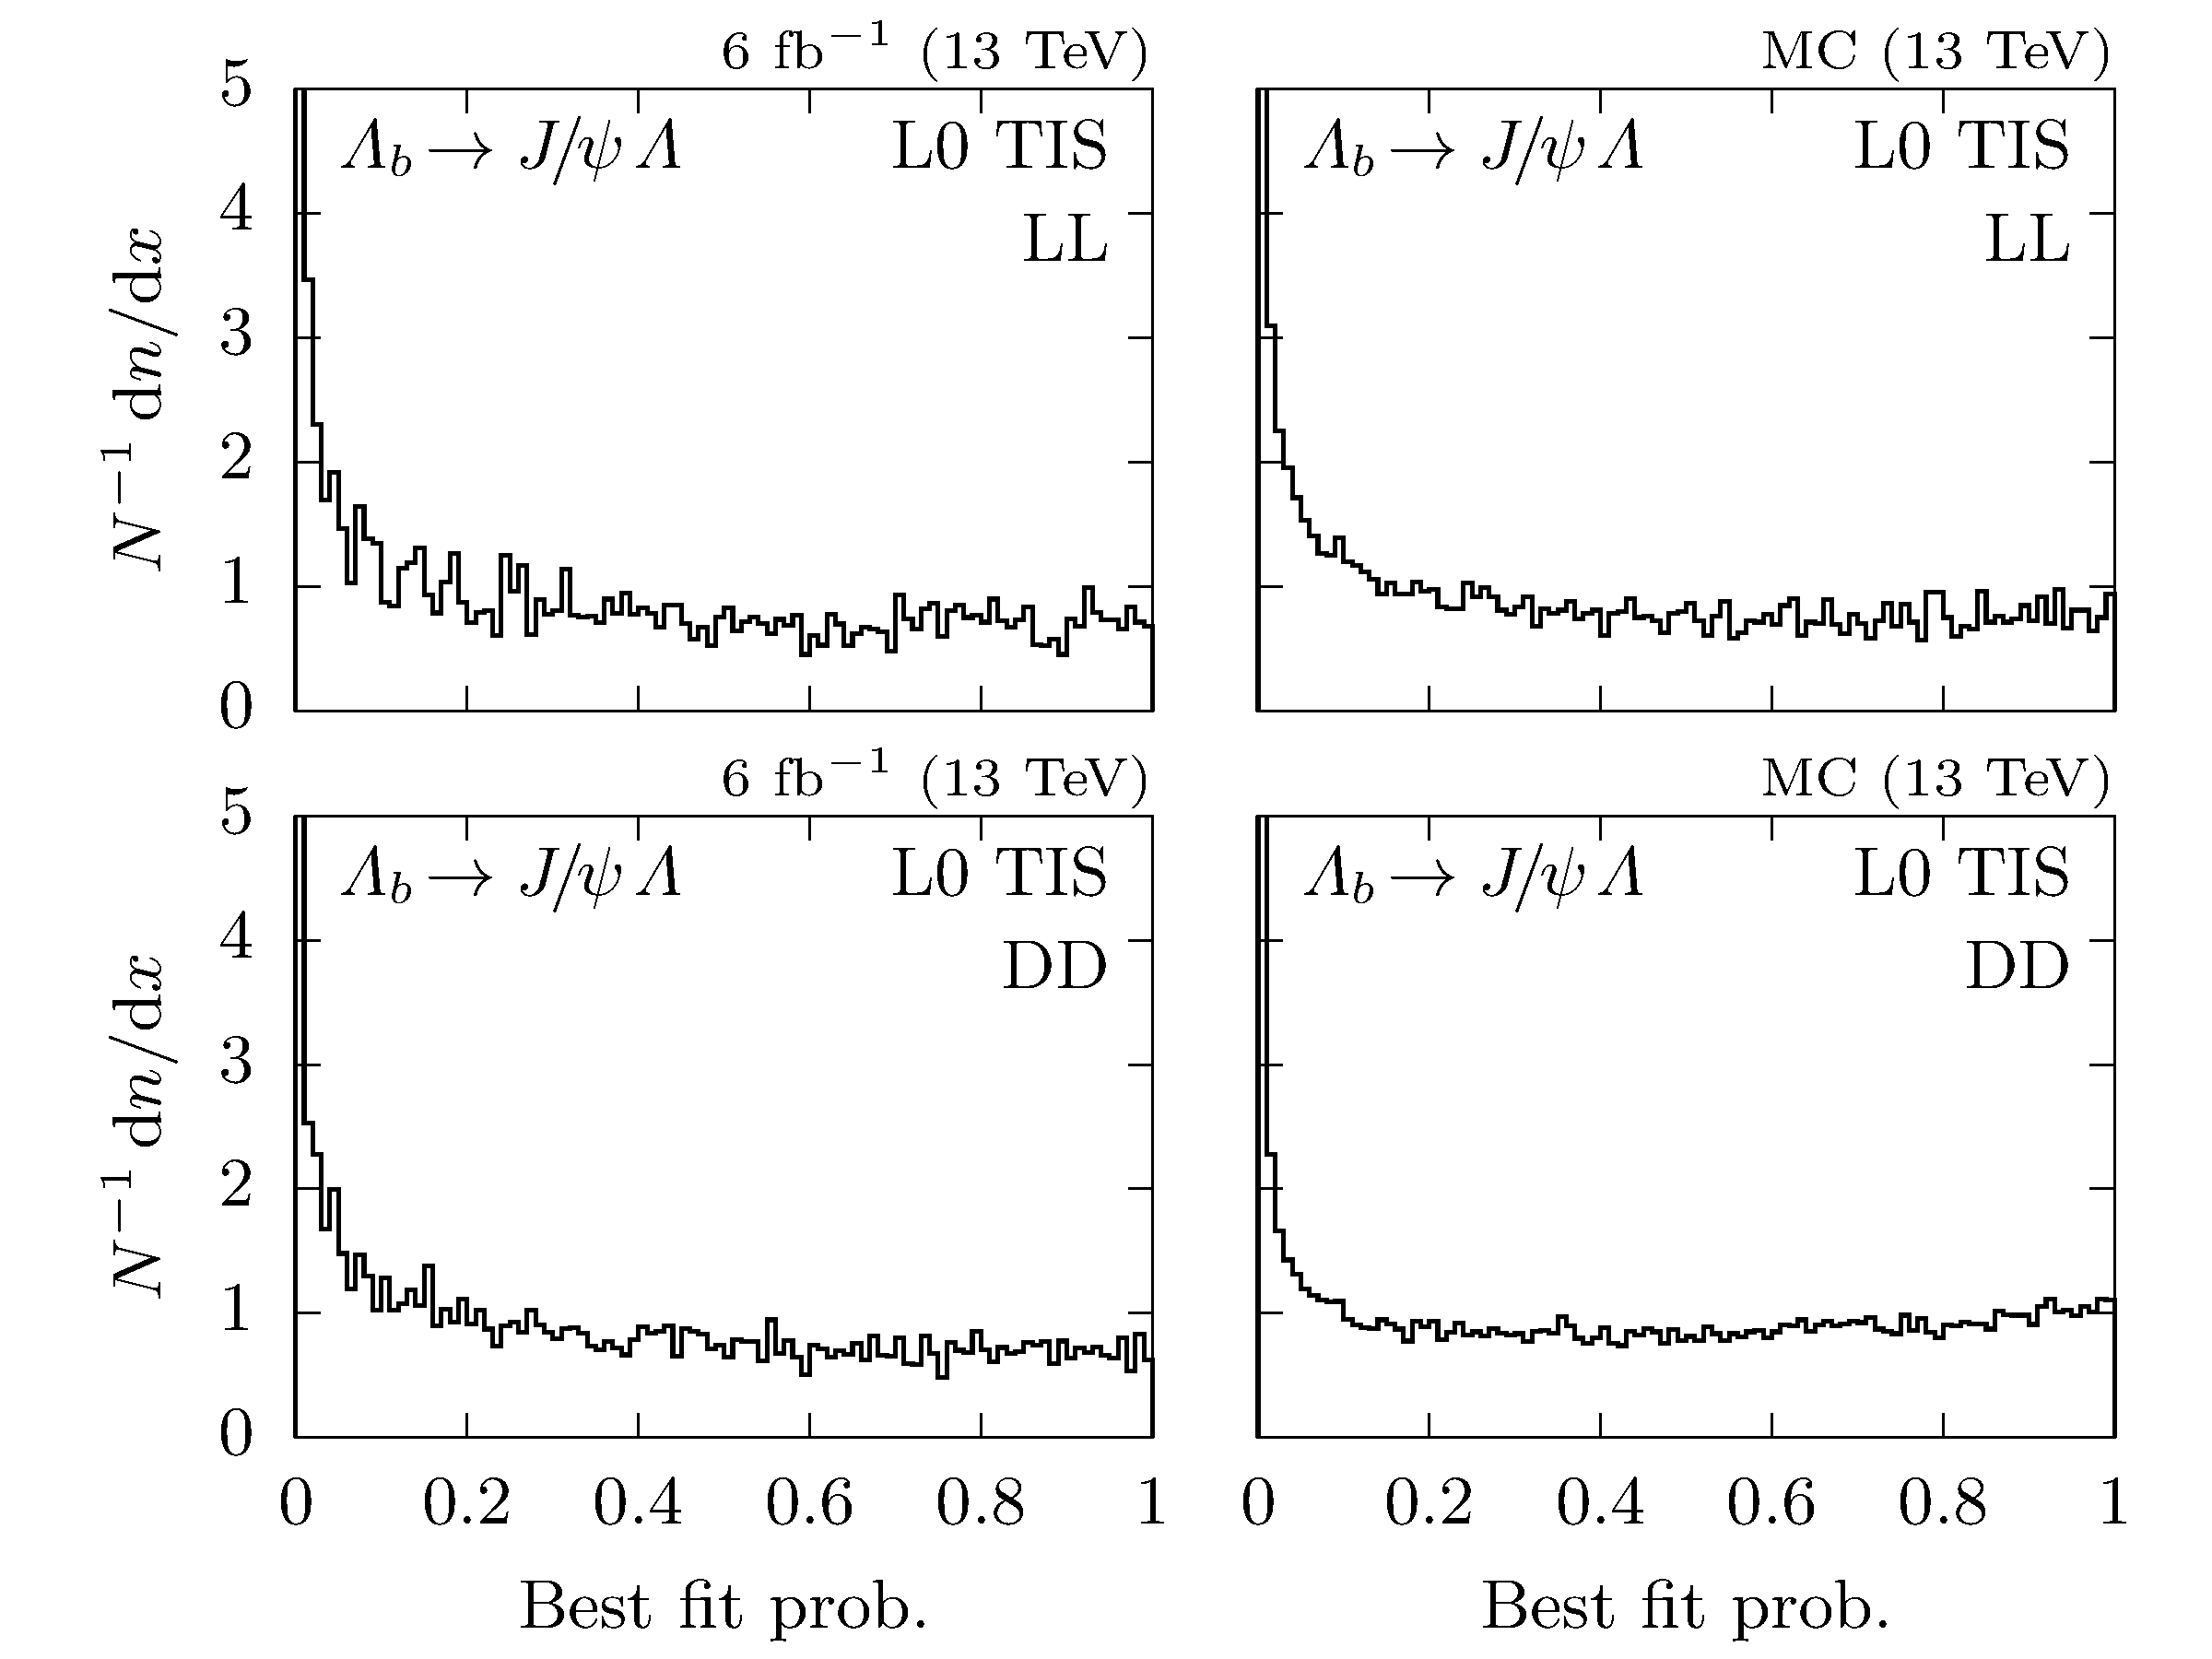
\includegraphics[scale=1.]{Lb2JpsiLz_weighting/hfitProb.png}
    \caption{Fit probability of \gls{LL} and \gls{DD} tracks (top and bottom), and for recorded data (left) and \gls{truthmatched}, simulated events (right).}
    \label{fig:fitprob_LbToJpsiLz}
\end{figure}

